\documentclass[fleqn, 11pt]{article}
\usepackage{float}
\usepackage{graphicx}
\usepackage[portuges]{babel}
\usepackage[utf8x]{inputenc}
\usepackage{comment}
\usepackage{fullpage}
\usepackage{xcolor}
\usepackage{amsmath,amsfonts,amssymb,amsthm, bm}

\usepackage{listings}
\usepackage{color}
\definecolor{mygreen}{RGB}{28,172,0}
\definecolor{mylilas}{RGB}{170,55,241}
\renewcommand{\min}{\expandafter\,\operatorname*{min}}

\begin{document}
\noindent
\large\textbf{Trabalho 4} \hfill \textbf{Luis Vinicius Costa Silva} \\
\normalsize Sistemas Bioinspirados \\
Prof. Fran Sérgio Lobato \\
\hfill Data de Entrega: 08/06/2019

\section*{Introdução}
Os problemas a seguir foram resolvidos utilizando o método do Recozimento Simulado com os seguintes parâmetros:

\begin{itemize}
\item chute inicial de $x = (0.8, 0.8)$;
\item $500$ temperaturas;
\item temperatura inicial de $0.5$;
\item temperatura final de $0.01$;
\item tolerância de $10^{-5}$
\end{itemize}

Mais informações acerca das particularidades de execução do método podem ser encontradas nos arquivos anexos a este relatório.
\section{Questão 1}
Considere um peso de 500N suspenso por um cabo, como mostra a Figura \ref{figure:fig1}. Uma força $F = 100 N$ é aplicada no peso. Sob o efeito dessa força, o peso move-se da posição original $A$ para uma nova posição de equilíbrio $B$. A posição de equilíbrio é tal que a energia potencial $PE$ é mínima, onde $PE = WY-FX$ e $x = L \sin (\theta)$ e $y = L(1 - \cos \theta)$.

\begin{figure}[!htb]
\label{figure:fig1}
   \center{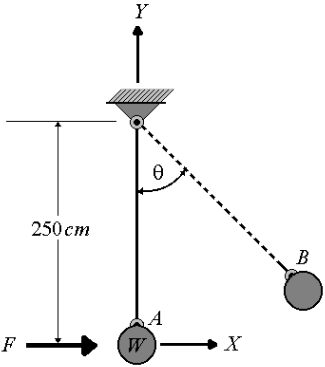
\includegraphics[width=0.33\textwidth]{pendulo.png}}
   \caption{O dito pêndulo}
\end{figure}

A posição de equílibrio do pêndulo que corresponde a energia potencial mínima é descrita da seguinte forma:

\begin{align*}
x^2 + (2.5 - y)^2 = 2.5^2 \tag*{Aplica-se o teorema de Pítagoras} \\
y = 2.5 - \sqrt{6.25 - x^2} \\
{min}_{x}\text{\phantom{0}} 500 (2.5 - \sqrt{6.25-x^2})-100x)
\end{align*}
Através da execução do algoritmo de Recozimento Simulado temos que ${min}_{x} = (0.49551,-24.752)$, coincidindo com o resultado analítico:
\begin{align*}
{min}_{x} = \bigg ( \frac{5}{2 \sqrt{26}}, -250 (\sqrt{26}-5) \bigg )
\end{align*}

A figura \ref{figure:fig2} descreve a mudança do ${min}_{f(x)}$ computado através da função objetivo descrita anteriormente utilizando o Recozimento Simulado:

\begin{figure}[!htb]
\label{figure:fig2}
   \center{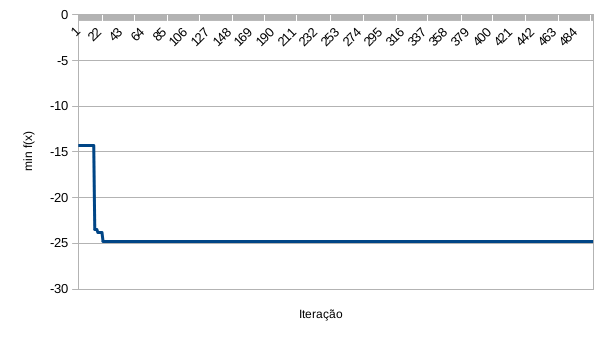
\includegraphics[width=0.8\textwidth]{convergencia_1.png}}
   \caption{Convergência do ${min}_{f(x)}$ durante a execução do Recozimento Simulado.}
\end{figure}

\section{Questão 2}
Observe a figura \ref{figure:fig3}:
\begin{figure}[H]
\label{figure:fig3}
   \center{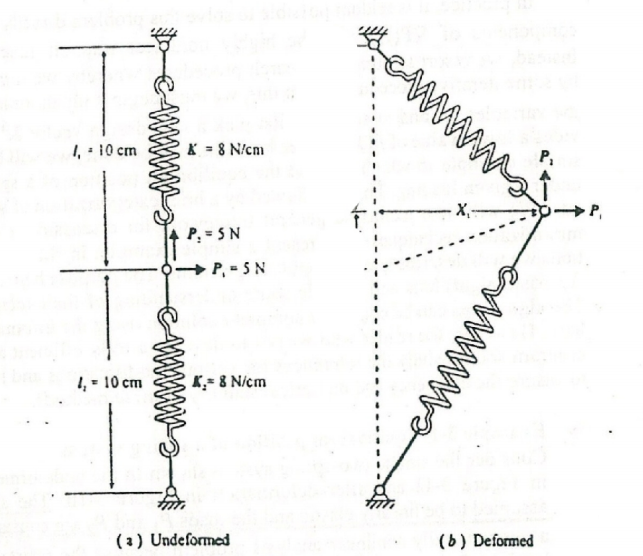
\includegraphics[width=0.5\textwidth]{molas.png}}
   \caption{Sistema de molas}
\end{figure}
Considerando que as molas são linearmente elásticas com cargas $P_1$ e $P_2$ constantes, temos que a energia potencial mínima do sistema é dada por:

\begin{align*}
E_p = \frac{1}{2}K_1(\Delta l_1)^2 + \frac{1}{2} K_2(\Delta l_2)^2 - P_1 X_1 - P_2 X_2
\end{align*}

onde $\Delta l_1$ e $\Delta l_2$ são as deformações lineares de suas respectivas molas. Reescrevendo a equação acima em termos de $x_1$ e $x_2$ temos:

\begin{align*}
E_p = \frac{1}{2}K_1 \bigg (\sqrt{x_1^2+(l_1-x_2)^2}-l_1 \bigg ) ^2 + \frac{1}{2} K_2 \bigg (\sqrt{x_1^2+(l_2-x_2)^2}-l_2 \bigg ) ^2 - P_1 X_1 - P_2 X_2
\end{align*}

Através da execução do algoritmo de Recozimento Simulado temos que ${min}_{x} = (8.6217, 4.5304, -41.8079)$, aproximando o resultado analítico de maneira satisfatória.

A figura \ref{figure:fig4} descreve a mudança do ${min}_{f(x)}$ computado através da função objetivo descrita anteriormente utilizando o Recozimento Simulado:

\begin{figure}[!htb]
\label{figure:fig4}
   \center{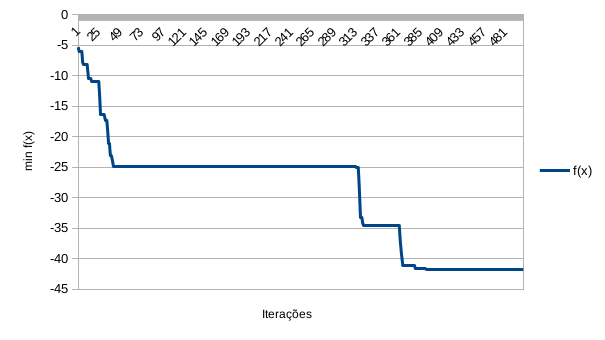
\includegraphics[width=0.8\textwidth]{convergencia_2.png}}
   \caption{Convergência do ${min}_{f(x)}$ durante a execução do Recozimento Simulado.}
\end{figure}
\end{document}